\newpage
\section{TỌA ĐỘ CỦA VECTƠ TRONG KHÔNG GIAN}
\subsection{LÝ THUYẾT CẦN NHỚ}
\subsubsection{Hệ tọa độ trong không gian}
\indam{Định nghĩa:}
\begin{boxdn}
	\immini{Trong không gian, cho ba trục $Ox$, $Oy$, $Oz$ đôi một vuông góc. Gọi $\overrightarrow{i}$, $\overrightarrow{j}$, $\overrightarrow{k}$ lần lượt là ba vectơ đơn vị trên các trục $Ox$, $Oy$, $Oz$. Hệ ba trục như vậy được gọi là \textit{\textbf{hệ trục tọa độ Descartes vuông góc Oxyz}} trong không gian hay gọi đơn giản là \textit{\textbf{hệ tọa độ Oxyz}}.}
	{	\begin{tikzpicture}[scale=0.6, font=\footnotesize,line join=round, line cap=round, >=stealth]
			\path
			(0,0) coordinate (A)
			++(-130:3) coordinate (B)
			++(0:4) coordinate (C)
			($(A)+(C)-(B)$) coordinate (D)
			;
			\foreach \i in {A,B,C,D}{
				\coordinate (\i') at ($(\i)+(0,4)$);
			}
			\coordinate (M) at ($(C')!0.5!(D')$);
			\draw (B)--(A)--(D) (A)--(A');
			\draw[dashed](A)--(0,-3) (A)--(-3,0) (A)--(1.7,2);
			\draw [red,->,thick](A)--++(-130:1)node[left]{$\overrightarrow {i}$};
			\draw [red,->,thick](A)--++(0:1)node[below]{$\overrightarrow {j}$};
			\draw [red,->,thick](A)--++(90:1)node[left]{$\overrightarrow {k}$};
			\draw [->](B)--++(-130:1)node[right]{$x$};
			\draw [->](D)--++(0:1)node[below]{$y$};
			\draw [->](A')--++(90:1)node[left]{$z$};
	\end{tikzpicture}}
\end{boxdn}
\begin{khung4}{Nhận xét}
	\begin{enumerate}
		\item 
		\begin{itemize}
			\item Điểm $O$ được gọi là \textbf{gốc tọa độ}.
			\item Các mặt phẳng $(Oxy)$, $(Oyz)$, $(Oxz)$ đôi một vuông góc với nhau gọi là các \textit{\textbf{mặt phẳng tọa độ}}.
			\item Không gian với hệ tọa độ $Oxyz$ còn được gọi là \textit{\textbf{không gian}} $Oxyz$.
		\end{itemize}
		\item Vì $\overrightarrow{i}$, $\overrightarrow{j}$, $\overrightarrow{k}$ là ba vectơ đơn vị đôi một vuông góc với nhau nên ta có
		\[\overrightarrow{i}^2=\overrightarrow{j}^2=\overrightarrow{k}^2=1\ \text{và}\ \overrightarrow{i}\cdot\overrightarrow{j}=\overrightarrow{j}\cdot\overrightarrow{k}=\overrightarrow{k}\cdot\overrightarrow{i}=0.\]
	\end{enumerate}
\end{khung4}
\subsubsection{Tọa độ của điểm và vectơ}
\begin{itemize}
	\item \textbf{Tọa độ của điểm}
	\begin{khung4}{}
			\immini{Trong không gian $Oxyz$, cho điểm $M$. Nếu $\overrightarrow{OM}=x\overrightarrow{i}+y\overrightarrow{j}+z\overrightarrow{k}$ thì ta gọi bộ ba số $(x;y;z)$ là \textit{\textbf{tọa độ của điểm}} $M$ đối với hệ trục tọa độ $Oxyz$ và viết $M=(x;y;z)$ hoặc $M(x;y;z)$; $x$ là hoành độ, $y$ là tung độ, $z$ là cao độ của điểm $M$.}
		{		\begin{tikzpicture}[line join = round, line cap=round,>=stealth,font=\footnotesize,scale=1]
				\path 
				(0,0) coordinate (O)
				(-2,-2) coordinate (A')
				(4,0) coordinate (B')
				(0,3) coordinate (C')
				($(O)!0.3!(C')$) coordinate (C1)
				($(O)!0.3!(B')$) coordinate (B1)
				($(O)!0.3!(A')$) coordinate (A1)
				($(O)!0.8!(C')$) coordinate (C)
				($(O)!0.8!(B')$) coordinate (B)
				($(O)!0.8!(A')$) coordinate (A)
				;
				
				\foreach \diem/\t/\r in{A'/x/-90,
					B'/y/60,
					C'/z/60,
					A1/\overrightarrow{i}/-60,
					B1/\overrightarrow{j}/-90,
					C1/\overrightarrow{k}/180} 
				\draw[->,line width=1pt] (O)--(\diem)node[shift={(\r:4mm)},scale=1.2]{$\t$};
				
				\draw[dashed] 
				(A)--($(A)+(B)-(O)$) coordinate (H) --(B)
				(C)--($(C)+(H)-(O)$)coordinate (M) node[above=0.2cm]{$M$}--(H)
				(H)--(O)--(M);
				
				\draw (M);
				\draw pic[draw,angle radius=3mm] {right angle = O--A--H}; 
				\draw pic[draw,angle radius=3mm] {right angle = O--B--H}; 
				\draw pic[draw,angle radius=3mm] {right angle = O--C--M}; 
				\draw[cyan,line width=2pt,->] (O)--(M); 
				
				\foreach \p/\r in {O/160}
				\fill (\p) circle (1.2pt) node[shift={(\r:3mm)}]{$\p$};
		\end{tikzpicture}}
	\end{khung4}
	\item \textbf{Tọa độ của vectơ}
	\begin{khung4}{}
		Trong không gian $Oxyz$, cho vectơ 
			$\overrightarrow{a}$. Nếu $\overrightarrow{a}=a_1\overrightarrow{i}+a_2\overrightarrow{j}+a_3\overrightarrow{k}$ thì ta gọi bộ ba số $(a_1;a_2;a_3)$ là \textit{\textbf{tọa độ của vectơ}} $\overrightarrow{a}$ đối với hệ tọa độ $Oxyz$ và viết $\overrightarrow{a}=(a_1;a_2;a_3)$ hoặc $\overrightarrow{a}(a_1;a_2;a_3)$.
	\end{khung4}
	\begin{khung4}{Nhận xét}
	Trong không gian $Oxyz$ ta có
	\begin{itemize}
		\item Tọa độ của điểm $M$ là tọa độ của vectơ $\overrightarrow{OM}$ tức là
		\[M=(x;y;z)\Leftrightarrow \overrightarrow{OM}=(x;y;z).\]
		\item Điều kiện để hai vectơ bằng nhau:\\
		Cho $\overrightarrow{u}=(x_1;y_1;z_1)$ và $\overrightarrow{v}=(x_2;y_2;z_2)$. Khi đó
		\[\overrightarrow{u}=\overrightarrow{v}\Leftrightarrow\heva{&x_1=x_2\\&y_1=y_2\\&z_1=z_2.}\]
	\end{itemize}
	\end{khung4}
	\end{itemize}
%-------------------------------------------------------------------------------------------------------------
\subsection{PHÂN LOẠI VÀ PHƯƠNG PHÁP GIẢI TOÁN}
\begin{dang}{Tìm tọa độ của điểm}
	\textit{Phương pháp: Sử dụng lý thuyết về tọa độ điểm}.
\end{dang}
\begin{vd}%[2H2N2-2]%[Dự án đề cương 3 khối NH24-25 - Đợt 2 - Lê Phúc]
	Cho hình hộp chữ nhật $OABC.O'A'B'C'$ có cạnh $OA=4$, $OC=6$, $OO'=3$. Chọn hệ trục tọa độ $Oxyz$ có gốc tọa độ $O$, các điểm $A$, $C$, $O'$ lần lượt nằm trêm các tia $Ox$, $Oy$, $Oz$. Xác định tọa độ các điểm $A$, $B$, $B'$.
	\loigiai{
		\begin{itemize}
			\item $\overrightarrow{OA}=4\overrightarrow{i}+0\overrightarrow{j}+0\overrightarrow{k}$, suy ra $A(4;0;0)$.
			\item $\overrightarrow{OB}=\overrightarrow{OA}+\overrightarrow{OC}=4\overrightarrow{i}+6\overrightarrow{j}+0\overrightarrow{k}$, suy ra $B(4;6;0)$.
			\item $\overrightarrow{OB'}=\overrightarrow{OA}+\overrightarrow{OC}+\overrightarrow{OD'}=4\overrightarrow{i}+6\overrightarrow{j}+3\overrightarrow{k}$, suy ra $A(4;6;3)$.
	\end{itemize}}
\end{vd}
\begin{dang}{Tìm tọa độ vectơ}
	\textit{Phương pháp: Sử dụng lý thuyết về tọa độ vectơ}.
\end{dang}
\setcounter{vd}{0}
\begin{vd}%[2H2N2-3]%[Dự án đề cương 3 khối NH24-25 - Đợt 1 - Lê Phúc]
	Trong không gian $Oxyz$ biết 
	$\overrightarrow{a}=5\overrightarrow{i}+7\overrightarrow{j}-3\overrightarrow{k}$, $\overrightarrow{b}=2\overrightarrow{i}+4\overrightarrow{k}$. Tìm tọa độ các vectơ $\overrightarrow{a}$, $\overrightarrow{b}$.
	\loigiai{
		\begin{itemize}
			\item $\overrightarrow{a}=5\overrightarrow{i}+7\overrightarrow{j}-3\overrightarrow{k}=(5;7;-3)$.
			\item $\overrightarrow{b}=2\overrightarrow{i}+4\overrightarrow{k}=(2;0;4)$.
		\end{itemize}
	}
\end{vd}
\begin{vd}%[2H2N2-3]%[Dự án đề cương 3 khối NH24-25 - Đợt 2 - Lê Phúc]
	Trong không gian $Oxyz$ biết $A(7;-2;1)$, $B(0;5;0)$. Tính $\overrightarrow{OA}$, $\overrightarrow{OB}$ theo các vectơ $\overrightarrow{i}$, $\overrightarrow{j}$, $\overrightarrow{k}$.
	\loigiai{
		\begin{itemize}
			\item $\overrightarrow{OA}=(7;2;-1)=7\overrightarrow{i}+2\overrightarrow{j}-\overrightarrow{k}$.
			\item $\overrightarrow{OB}=(0;5;0)=5\overrightarrow{j}$.
		\end{itemize}
	}
\end{vd}
\begin{vd}%[2H2H2-3]%[Dự án đề cương 3 khối NH24-25 - Đợt 2 - Lê Phúc]
	Trong không gian $Oxyz$ cho hình hộp chữ nhật $ABCD.A'B'C'D'$ có đỉnh $A$ trùng với gốc $O$, các vectơ $\overrightarrow{AB}$, $\overrightarrow{AD}$, $\overrightarrow{AA'}$ theo thứ tự cùng hướng với vectơ $\overrightarrow{i}$, $\overrightarrow{j}$, $\overrightarrow{k}$ và có $AB=8$, $AD=6$, $AA'=4$. Tìm tọa độ các vectơ $\overrightarrow{AB}$, $\overrightarrow{AC}$, $\overrightarrow{AC'}$ và $\overrightarrow{AM}$ với $M$ là trung điểm của cạnh $C'D'$.
	\begin{center}
		\begin{tikzpicture}[scale=0.6, font=\footnotesize,line join=round, line cap=round, >=stealth]
		\path
		(0,0) coordinate (A)
		++(-130:3) coordinate (B)
		++(0:4) coordinate (C)
		($(A)+(C)-(B)$) coordinate (D)
		;
		\foreach \i in {A,B,C,D}{
			\coordinate (\i') at ($(\i)+(0,4)$);
		}
			\coordinate (M) at ($(C')!0.5!(D')$);
		\draw (A')--(B')--(C')--(D')--cycle
		(B')--(B)--(C)--(C')  (C)--(D)--(D');
		\draw [red,->,thick](A)--++(-130:1)node[left]{$\overrightarrow {i}$};
		\draw [red,->,thick](A)--++(0:1)node[below]{$\overrightarrow {j}$};
		\draw [red,->,thick](A)--++(90:1)node[left]{$\overrightarrow {k}$};
		\draw [->,thick](B)--++(-130:1)node[right]{$x$};
		\draw [->,thick](D)--++(0:1)node[below]{$y$};
		\draw [->,thick](A')--++(90:1)node[left]{$z$};
		\draw[dashed,thin](A)--(B)(A)--(D)(A)--(A')
		[->](A)--(C')
		;
		\foreach \i/\g in {A'/45,B'/90,C'/-30,D'/45,A/180,B/180,C/-90,D/-90,M/-30}
		\fill[black] (\i) circle(1pt)+(\g:5mm)node[scale=1]{$\i$};
	\end{tikzpicture}
\end{center}
	\loigiai{
	Để tìm tọa độ của vectơ $\overrightarrow{AB}$, ta cần biểu diễn $\overrightarrow{AB}$ theo ba vectơ $\overrightarrow{i}$, $\overrightarrow{j}$, $\overrightarrow{k}$.\\
	Do $\overrightarrow{AB}$ cùng hướng với $\overrightarrow{i}$ và $\left|\overrightarrow{AB}\right|=AB=8=8\left|\overrightarrow{i}\right|$ nên 
	\[\overrightarrow{AB}=8\overrightarrow{i}\ \text{hay}\ \overrightarrow{AB}=8\overrightarrow{i}+0\overrightarrow{j}+0\overrightarrow{k}.\]
	Tương tự ta có $\overrightarrow{AD}=0\overrightarrow{i}+6\overrightarrow{j}+0\overrightarrow{k}$, $\overrightarrow{AA'}=0\overrightarrow{i}+0\overrightarrow{j}+4\overrightarrow{k}$.
	\begin{itemize}
		\item Trong hình hình hành $ABCD$ ta có $\overrightarrow{AC}=\overrightarrow{AB}+\overrightarrow{AD}=8\overrightarrow{i}+6\overrightarrow{j}+0\overrightarrow{k}$.
		\item Trong hình hình hành $AA'C'C$ ta có $\overrightarrow{AC'}=\overrightarrow{AC}+\overrightarrow{AA'}=8\overrightarrow{i}+6\overrightarrow{j}+4\overrightarrow{k}$.
	\end{itemize}
	Suy ra $\overrightarrow{AB}=(8;0;0)$; $\overrightarrow{AC}=(8;6;0)$; $\overrightarrow{AC'}=(8;6;4)$.\\
	Ta có
	\begin{eqnarray*}
	\overrightarrow{AM}&=&\dfrac{1}{2}\left(\overrightarrow{AC'}+\overrightarrow{AD'}\right)=\dfrac{1}{2}\left(\overrightarrow{AC'}+\overrightarrow{AD}+\overrightarrow{AA'}\right)\\
	&=&\dfrac{1}{2}\left(8\overrightarrow{i}+6\overrightarrow{j}+4\overrightarrow{k}+6\overrightarrow{j}+4\overrightarrow{k}\right)\\
	&=&4\overrightarrow{i}+6\overrightarrow{j}+4\overrightarrow{k}.
	\end{eqnarray*} 
	Vậy $\overrightarrow{AM}=(4;6;4)$.
}
\end{vd}
\begin{dang}{Ứng dụng}
	\textit{Phương pháp: Mô hình các bài toán thực tiễn thành các bài toán về tọa độ vectơ hoặc tọa độ điểm}.
\end{dang}
\setcounter{vd}{0}
\begin{vd}%[2D4V1-6]%[Dự án đề cương 3 khối NH24-25 - Đợt 2 - Lê Phúc]
	(\textit{Trích đề thi CKI - THPT Phan Ngọc Hiển - Năm học 2024-2025})\\
	Ở một sân bay, vị trí của máy bay được xác định bởi điểm $P$ trong không gian $Oxyz$ (như hình vẽ).
	Gọi $H$ là hình chiếu vuông góc của $P(a;b;c)$ xuống mặt phẳng $(Oxy)$. Cho biết $OP=41$, $\left(\overrightarrow{i},\overrightarrow{OH}\right)=52^{\circ}$, $\left(\overrightarrow{OH},\overrightarrow{OP}\right)=46^{\circ}$. Tính giá trị của biểu thức $S=a+b+c$ (kết quả làm tròn đến hàng phần mười).
	\begin{center}
		\begin{tikzpicture}[line join = round, line cap=round,>=stealth,font=\footnotesize,scale=1]
			\path 
			(0,0) coordinate (O)
			(-2,-2) coordinate (A')
			(4,0) coordinate (B')
			(0,3) coordinate (C')
			($(O)!0.3!(C')$) coordinate (C1)
			($(O)!0.3!(B')$) coordinate (B1)
			($(O)!0.3!(A')$) coordinate (A1)
			($(O)!0.8!(C')$) coordinate (C)
			($(O)!0.8!(B')$) coordinate (B)
			($(O)!0.8!(A')$) coordinate (A)
			;
			
			\foreach \diem/\t/\r in{A'/x/-90,
				B'/y/60,
				C'/z/60,
				A1/\overrightarrow{i}/-60,
				B1/\overrightarrow{j}/-90,
				C1/\overrightarrow{k}/180} 
			\draw[->,line width=1pt] (O)--(\diem)node[shift={(\r:4mm)},scale=1.2]{$\t$};
			
			\draw[dashed] 
			(A)--($(A)+(B)-(O)$) coordinate (H) --(B)
			(C)--($(C)+(H)-(O)$)coordinate (P) node[above=0.5cm]{$P$}--(H)
			(H)--(O)--(P);
			
			\draw (P);
			\draw pic[draw,angle radius=3mm] {right angle = O--A--H}; 
			\draw pic[draw,angle radius=3mm] {right angle = O--B--H}; 
			\draw pic[draw,angle radius=3mm] {right angle = O--C--P}; 
			\draw[cyan,line width=2pt,->] (O)--(P); 
			
			\foreach \p/\r in {A/160,B/90,C/180,H/-45,O/160}
			\fill (\p) circle (1.2pt) node[shift={(\r:3mm)}]{$\p$};
		\end{tikzpicture}
	\end{center}
	
	\loigiai{Ta có $OC=PH=OP \cdot \sin \left(\overrightarrow{OH}, \overrightarrow{OP}\right)=41 \cdot \sin 46^{\circ} \approx 29{,}49$.\\
		$OH=OP \cdot \cos \left(\overrightarrow{OH}, \overrightarrow{OP}\right)=41 \cdot \cos 46^{\circ}\approx 28{,}48$. \\
		$OA=OH \cdot \cos \left(\overrightarrow{i}, \overrightarrow{OH}\right)=28{,}48 \cdot \cos 52^{\circ}\approx 17{,}53$.\\
		$OB=OH \cdot \cos \left(90^{\circ}-\left(\overrightarrow{i}, \overrightarrow{OH}\right)\right)=28{,}48 \cdot \cos \left(90^{\circ}-52^{\circ}\right)=28{,}48 \cdot \cos 38^{\circ} \approx 17{,}71$.\\
		Suy ra $M(17{,}53;17{,}71;29{,}49)$ $\Rightarrow S=a+b+c=17{,}53+17{,}71+29{,}49=64{,}73 \approx 64{,}7$.
	}
\end{vd}
%-----------------------------------------------------------------------------
\subsection{Bài tập rèn luyện}
\ind{PHẦN I.} \inden{Câu trắc nghiệm nhiều phương án lựa chọn. Mỗi câu hỏi học sinh chỉ chọn một phương án.}\\
\setcounter{ex}{0}
\Opensolutionfile{ans}[ans/2D1-Bai1-TN]%--Đặt tên 2D1-Bai1-Dang1-TN
\begin{ex}%[2H2N2-3]%[Dự án đề cương 3 khối NH24-25 - Đợt 2 - Lê Phúc]
	Trong không gian với hệ trục tọa độ $Oxyz$, cho vectơ $\overrightarrow{a}=(0;-3;2)$. Mệnh đề nào sau đây \textbf{đúng}?
	\choice
	{\True $\overrightarrow{a}=-3\overrightarrow{j}+2\overrightarrow{k}$}
	{$\overrightarrow{a}=-3\overrightarrow{i}+2\overrightarrow{k}$}
	{$\overrightarrow{a}=-3\overrightarrow{i}+2\overrightarrow{j}+\overrightarrow{k}$}
	{$\overrightarrow{a}=-3\overrightarrow{i}+2\overrightarrow{j}$}
	\loigiai{
	Do $\overrightarrow{a}=(0;-3;2)$ nên $\overrightarrow{a}=-3\overrightarrow{j}+2\overrightarrow{k}$.
	}
\end{ex}
\begin{ex}%[2H2N2-2]%[Dự án đề cương 3 khối NH24-25 - Đợt 2 - Lê Phúc]
	Trong không gian $Oxyz$, cho điểm $M$ thỏa mãn hệ thức $\overrightarrow{OM}=\overrightarrow{i}-5\overrightarrow{j}+2\overrightarrow{k}$. Tọa độ điểm $M$ là
	\choice
	{$(2;5;1)$}
	{\True $(1;-5;2)$}
	{$(2;-5;1)$}
	{$(1;5;2)$}
	\loigiai{
	Tọa độ điểm $M$ thỏa mãn hệ thức $\overrightarrow{OM}=\overrightarrow{i}-5\overrightarrow{j}+2\overrightarrow{k}$ là $(1;-5;2)$.
	}
\end{ex}
\begin{ex}%[2H2N2-2]%[Dự án đề cương 3 khối NH24-25 - Đợt 2 - Lê Phúc]
	Trong không gian $Oxyz$, cho điểm $M(1; -2; 1)$. Tọa độ của vectơ $\overrightarrow{OM}$ là
	\choice
	{\True $(1;-2; 1)$}
	{$(1;2;1)$}
	{$(-1;2;-1)$}
	{$(1;2;-1)$}
	\loigiai{
		Ta có $\overrightarrow{OM}=(1; 2;-1)$.
	}
\end{ex}
\begin{ex}%[2H2N2-3]%[Dự án đề cương 3 khối NH24-25 - Đợt 2 - Lê Phúc]
	(\textit{Trích đề thi CKI - Trường THPT Tân Châu - Năm học 2024-2025})\\
	Trong không gian $Oxyz$, cho điểm $A(-2; 3; 5)$. Tọa độ của vectơ $\overrightarrow{OA}$ là
	\choice
	{$(2;-3; 5)$}
	{$(2;-3;-5)$}
	{\True $(-2; 3; 5)$}
	{$(-2;-3; 5)$}
	\loigiai{
		Ta có $\overrightarrow{OA}=(-2; 3; 5)$.
	}
\end{ex}
\begin{ex}%[2H2N2-3]%[Dự án đề cương 3 khối NH24-25 - Đợt 2 - Lê Phúc]
	(\textit{Trích đề thi CKI - Trường THPT Trần Phú - Năm học 2024-2025})\\
	Trong không gian $Oxyz$, cho điểm $N(2; 4;-7)$. Tính vectơ $\overrightarrow{ON}$ theo các vectơ $\overrightarrow{i}$, $\overrightarrow{j}$, $\overrightarrow{k}$.
	\choice
	{\True $\overrightarrow{ON}=2 \overrightarrow{i}+4 \overrightarrow{j}-7 \overrightarrow{k}$}
	{$\overrightarrow{ON}=4 \overrightarrow{i}-2 \overrightarrow{j}+7 \overrightarrow{k}$}
	{$\overrightarrow{ON}=2 \overrightarrow{i}+7 \overrightarrow{j}-4 \overrightarrow{k}$}
	{$\overrightarrow{ON}=2 \overrightarrow{i}-4 \overrightarrow{j}+7 \overrightarrow{k}$}
	\loigiai{
		Do $N(2; 4;-7)$ nên $\overrightarrow{ON}=(2;-4;-7)$, hay $\overrightarrow{ON}=2 \overrightarrow{i}+4 \overrightarrow{j}-7 \overrightarrow{k}$.
	}
\end{ex}
\begin{ex}%[2H2N2-2]%[Dự án đề cương 3 khối NH24-25 - Đợt 2 - Lê Phúc]
	(\textit{Trích đề thi CKI - Trường THPT Chuyên Lê Quý Đôn - Năm học 2024-2025})\\
	\immini{
		Tọa độ của điểm $P$ trong hình vẽ là
		\choice
		{$P(2;3;0)$}
		{\True $P(2;3;3)$}
		{$P(3;2;3)$}
		{$P(2;3;\sqrt{13}$)}
	}
	{
		\begin{tikzpicture}[scale=0.8,>=stealth, font=\footnotesize, line join=round, line cap=round]
			\draw[thick] (0,0)node[above left]{$O$}--(-150:4) (0,0)--(-30:4) (0,0)--(90:4);
			\draw[->,thick] (-150:4)--(-150:4.5)node[pos=1,below]{$x$};
			\draw[->,thick] (-30:4)--(-30:4.5)node[pos=1,below]{$y$};
			\draw[->,thick] (90:4)--(90:4.5)node[pos=1,above left]{$z$};
			\path
			($(-150:2)+(-30:3)+(90:3)$) coordinate (P)
			($(-150:2)+(-30:3)$) coordinate (H)
			(-150:2) coordinate (M)
			(-30:3) coordinate (N)
			($(P)+(M)-(H)$) coordinate (I)
			($(P)+(N)-(H)$) coordinate (K)
			(90:3) coordinate (J)
			;
			\foreach \x in {1,2,3,4}
			{
				\draw[gray!50] ($(-150:\x)+(0,4)$)--(-150:\x)--($(-150:\x)+(-30:4)$);
				\draw[gray!50] ($(-30:\x)+(0,4)$)--(-30:\x)--($(-30:\x)+(-150:4)$);
				\draw[gray!50] ($(-150:4)+(0,\x)$)--(90:\x)--($(-30:4)+(0,\x)$);
				\draw[fill=black](-150:\x)circle(1pt)node[above]{$\x$};
				\draw[fill=black](-30:\x)circle(1pt)node[above]{$\x$};
				\draw[fill=black](90:\x)circle(1pt)node[left]{$\x$};}
			\draw[fill=black] (P)node[below right]{$P$}circle(1pt);
			\draw[dashed] (I)--(M)--(H)--(P)--(I)--(J)--(K)--(P) (H)--(N)--(K);
		\end{tikzpicture}
	}
	\loigiai{
		Dựa vào hình vẽ, ta thấy tọa độ điểm $P(2;3;3)$.
	}
\end{ex}
\begin{ex}%[2H2N2-2]%[Dự án đề cương 3 khối NH24-25 - Đợt 2 - Lê Phúc]
	(\textit{Trích đề thi CKI - THPT Ngô Gia Tự - Năm học 2024-2025})\\
	Trong không gian $Oxyz$, xác định tọa độ của điểm $A$ biết $\vec{OA}=\vec{i}-5\vec{j}$.
	\choice
	{\True $(1;-5;0)$}
	{$(1;0;-5)$}
	{$(0;1;5)$}
	{$(1;5;0)$}
	\loigiai{
		Ta có $\vec{OA}=\vec{i}-5\vec{j}+0\vec{k}$ nên tọa độ của điểm $A$ là $(1;-5;0)$.
	}
\end{ex}
\begin{ex}%[2H2H2-2]%[Dự án đề cương 3 khối NH24-25 - Đợt 2 - Lê Phúc]
	(\textit{Trích đề thi CKI - THPT Ngô Gia Tự - Năm học 2024-2025})\\
	Trong không gian $Oxyz$, xác định tọa độ của điểm $A$ biết $\vec{OA}=\vec{i}-5\vec{j}$.
	\choice
	{$(1;5;0)$}
	{$(1;0;-5)$}
	{$(0;1;5)$}
	{\True $(1;-5;0)$}
	\loigiai{
		Ta có $\vec{OA}=\vec{i}-5\vec{j}+0\vec{k}$ nên tọa độ của điểm $A$ là $(1;-5;0)$.}
\end{ex}
\begin{ex}%[2H2N2-3]%[Dự án đề cương 3 khối NH24-25 - Đợt 2 - Lê Phúc]
	(\textit{Trích đề thi CKI - Trường PT DTNT - Năm học 2024-2025})\\
	Trong không gian $Oxy z$, cho $\overrightarrow{a}=-\overrightarrow{i}+2 \overrightarrow{j}-3 \overrightarrow{k}$. Tọa độ của vectơ $\overrightarrow{a}$ là
	\choice
	{\True $(-1 ; 2 ;-3)$}
	{$(2 ;-3 ;-1)$}
	{$(-3 ; 2 ;-1)$}
	{$(2 ;-1 ;-3)$}
	\loigiai{
		Tọa độ của vectơ $\overrightarrow{a}$ là $(-1;2-3)$.
	}
\end{ex}
\begin{ex}%[2H2H2-2]%[Dự án đề cương 3 khối NH24-25 - Đợt 2 - Lê Phúc]
	(\textit{Trích đề thi CKI - Trường THPT Trần Phú - Năm học 2024-2025})\\
	Trong không gian $Oxyz$, cho điểm $N(2; 4;-7)$. Tính vectơ $\overrightarrow{ON}$ theo các vectơ $\overrightarrow{i}$, $\overrightarrow{j}$, $\overrightarrow{k}$.
	\choice
	{$\overrightarrow{ON}=4 \overrightarrow{i}-2 \overrightarrow{j}+7 \overrightarrow{k}$}
	{$\overrightarrow{ON}=2 \overrightarrow{i}+7 \overrightarrow{j}-4 \overrightarrow{k}$}
	{\True $\overrightarrow{ON}=2 \overrightarrow{i}+4 \overrightarrow{j}-7 \overrightarrow{k}$}
	{$\overrightarrow{ON}=2 \overrightarrow{i}-4 \overrightarrow{j}+7 \overrightarrow{k}$}
	\loigiai{
		Do $N(2; 4;-7)$ nên $\overrightarrow{ON}=(2;-4;-7)$, hay $\overrightarrow{ON}=2 \overrightarrow{i}+4 \overrightarrow{j}-7 \overrightarrow{k}$.
	}
\end{ex}

\begin{ex}%[2H2N2-2]%[Dự án đề cương 3 khối NH24-25 - Đợt 2 - Lê Phúc]
	(\textit{Trích đề thi CKI - THPT Chuyên Lê Quý Đôn - Năm học 2024-2025})\\
		Trong không gian $Oxyz$, cho véc-tơ $\vec{u}=-3\vec{i}-2\vec{j}+3\vec{k}$. Tọa độ của véc-tơ $\vec{u}$ là bao nhiêu?
		\choice
		{$(-2;-3;3)$}
		{\True $(-3;-2;3)$}
		{$(3;-3;-2)$}
		{$(3;-2;3)$}
		\loigiai{
			Tọa độ của véc-tơ $\vec{u}$ là $(-3;-2;3)$.
		}
	\end{ex}
\begin{ex}%[2H2N2-2]%[Dự án đề cương 3 khối NH24-25 - Đợt 2 - Lê Phúc]
	Trong không gian $Oxyz$, cho $\overrightarrow{MO}=-\vec{i}+2\vec{j}-2\vec{k}$. Toạ độ của điểm $M$ là
	\choice
	{\True $(1;-2; 2)$}
	{$(-1; 2; -2)$}
	{$(1; 2; 2)$}
	{$(-1;-2; -2)$}
	\loigiai{
		Ta có $\overrightarrow{MO}=-\vec{i}+2\vec{j}-2\vec{k}\Leftrightarrow\overrightarrow{OM}=(1;-2;2)$ hay $M(1;-2;2)$.
	}
\end{ex}
\begin{ex}%[2H2N2-2]%[Dự án đề cương 3 khối NH24-25 - Đợt 2 - Lê Phúc]
	(\textit{Trích đề thi CKI - Trường THPT Lý Thường Kiệt - Năm học 2024-2025})\\
	Trong không gian với hệ trục tọa độ $Oxyz$, cho điểm $M$ thỏa $\overrightarrow{MO}=2\vec{j}-3\vec{i}+5\vec{k}$. Tọa độ của điểm $M$ là
	\choice
	{\True $M(3;-2;-5)$}
	{$M(-3;2;5)$}
	{$M(-2;3;-5)$}
	{$M(2;-3;5)$}
	\loigiai{
		Ta có $\overrightarrow{MO}=2\vec{j}-3\vec{i}+5\vec{k}$ suy ra $\overrightarrow{MO}=(-3;2;5) \Rightarrow \overrightarrow{OM}=(3;-2;-5)$.\\
		Vậy $M(3;-2;-5)$.
	}
\end{ex}


\begin{ex}%[2H2H2-2]%[Dự án đề cương 3 khối NH24-25 - Đợt 2 - Lê Phúc]
	(\textit{Trích đề thi CKI - THPT Thị Xã Quảng Trị - Năm học 2024-2025})\\
Trong không gian với hệ tọa độ $Oxyz$, cho điểm $A(1;2;3)$. Tọa độ của vectơ $\overrightarrow{OA}$ là
\choice
{$(0;2;3)$}
{$(1;2;0)$}
{$(1;0;3)$}
{\True $(1;2;3)$}
\loigiai{
	Ta có $\overrightarrow{OA}=(1;2;3)$.
	}
\end{ex}
\begin{ex}%[2H2H2-6]%[Dự án đề cương 3 khối NH24-25 - Đợt 2 - Lê Phúc]
	Trong không gian $Oxyz$, cho $\overrightarrow{MN}=3\overrightarrow{i}-2\overrightarrow{j}+4\overrightarrow{k}$. Tìm tọa độ véc-tơ $\overrightarrow{NM}$.
	\choice
	{$\overrightarrow{NM} = (3;-2;4)$}
	{$\overrightarrow{NM} = (3;2;4)$}
	{\True $\overrightarrow{NM} = (-3;2;-4)$}
	{$\overrightarrow{NM} = (-3;-2;-4)$}
	\loigiai{
		Ta có $\overrightarrow{NM}=-3\overrightarrow{i}+2\overrightarrow{j}-4\overrightarrow{k}$.\\
		Suy ra $\overrightarrow{NM}=(-3;2;-4)$.
	}
\end{ex}
\begin{ex}%[2H2V2-2]%[Dự án đề cương 3 khối NH24-25 - Đợt 2 - Lê Phúc]
	(\textit{Trích đề thi CKI - Trường THPT Duy Tân - Năm học 2024-2025})\\
	Trong không gian $Oxyz$, cho điểm $M$ xác định bởi $\overrightarrow{OM}=2\overrightarrow{i}+3\overrightarrow{j}+4\overrightarrow{k}$. Tọa độ điểm $M$ là
	\choice
	{\True $(2;3;4)$}
	{$(0;0;4)$}
	{$(0;3;0)$}
	{$(2;0;0)$}
	\loigiai{
		Tọa độ điểm $M$ là $(2;3;4)$.
	}
\end{ex}
\begin{ex}%[2H2H2-2]%[Dự án đề cương 3 khối NH24-25 - Đợt 2 - Lê Phúc]
	Cho hình lập phương $ABCD.A'B'C'D'$ có cạnh bằng  $1$. Lập hệ tọa độ $Oxyz$ có gốc $O$ trùng với đỉnh $B'$ và các vectơ đơn vị $\overrightarrow{i}$, $\overrightarrow{j}$, $\overrightarrow{k}$ lần lượt cùng chiều với các vectơ $\overrightarrow{B'A'}$, $\overrightarrow{B'C'}$, $\overrightarrow{B'B}$. Khi đó điểm $D$ có tọa độ là
	\choice
	{$D(1;0;0)$}
	{$D(0;1;1)$}
	{$D(0;1;0)$}
	{\True $D(1;1;1)$}
	\loigiai{
		$\overrightarrow{B'D}=\overrightarrow{B'A'}+\overrightarrow{B'C'}+\overrightarrow{B'B}=\overrightarrow{i}+\overrightarrow{j}+\overrightarrow{k}$.\\
		Suy ra $D(1;1;1)$.
	}
\end{ex}
\begin{ex}%[2H2H2-2]%[Dự án đề cương 3 khối NH24-25 - Đợt 2 - Lê Phúc]
	(\textit{Trích đề thi CKI - THPT Gia Định - Năm học 2024-2025})\\
	\immini{
		Cho hình chóp $S.ABCD$ có đáy là hình vuông cạnh bằng $4$, $SA=6$ và $SA \perp(ABCD)$. Chọn hệ trục $Oxyz$ có gốc tọa độ tại $A$; các điểm $B$, $D$, $S$ lần lượt trên các tia $Ox$, $Oy$, $Oz$. Biết tọa độ của điểm $C(a;b;c)$ Khi đó $a-b+4c$ bằng
		\choice
		{$4$}
		{\True $0$}
		{$-16$}
		{$16$}
	}
	{
		\begin{tikzpicture}[declare function={a=2.65;b=4.5;h=3;},line join=round,line cap=round,font=\footnotesize,>=stealth,scale=0.6]
			\path (0,0) coordinate (A)
			(-135:a) coordinate (B)
			(b,0) coordinate (D)
			($(D)-(A)+(B)$) coordinate (C)
			(0,h) coordinate (S)
			($(B)!-0.3!(A)$) coordinate (x)
			($(D)!-0.3!(A)$) coordinate (y)
			($(S)!-0.3!(A)$) coordinate (z)
			($(B)!.5!(C)$)  coordinate (E)
			;
			\draw[dashed] (S)--(A)--(B) (A)--(D);
			\draw (B)--(C)--(D) (B)--(S)  (D)--(S)--(C) ;
			\draw [->] (B)--(x)node[below]{$x$} ;
			\draw [->]  (D)--(y)node[right]{$y$};
			\draw [->]  (S)--(z)node[above]{$z$};
			\foreach \t/\g in {A/180,B/-90,C/-90,D/-60,S/120}{
				\draw[fill=black] (\t) circle (1pt) node[shift={(\g:7pt)},font=\scriptsize]{$ \t $};
			}
		\end{tikzpicture}
	}
	\loigiai{
		$\overrightarrow{AC}=\overrightarrow{AB}+\overrightarrow{AD}=4\overrightarrow{i}+4\overrightarrow{j}$.\\
		Suy ra $C(4;4;0)$.\\
		Vậy $a-b+4c=4-4+4\cdot 0=0$.
	}	
\end{ex}
\begin{ex}%[2H2N2-2]%[Dự án đề cương 3 khối NH24-25 - Đợt 2 - Lê Phúc]
	(\textit{Trích đề thi CKI - Trường THPT Chu Văn An - Năm học 2024-2025})\\
	\immini {
		Cho hình hộp chữ nhật $OABC.O'A'B'C'$ có cạnh $OA=4$, $OC=6$, $OO'=3$. Chọn hệ trục tọa độ $Oxyz$ có gốc tọa độ $O$; các điểm $A$, $C$, $O'$ lần lượt nằm trên các tia $Ox$, $Oy$, $Oz$. Xác định tọa độ điểm $B$?
		\choice[2]
		{$B(6;4;0)$}
		{\True $B(4;6;0)$}
		{$B(4;6;3)$}
		{$B(6;4;3)$}
	}{
		\begin{tikzpicture}[scale=0.6, font=\footnotesize,line join=round, line cap=round, >=stealth]
			\path
			(0,0) coordinate (O)
			++(-130:3) coordinate (A)
			++(0:4) coordinate (B)
			($(O)+(B)-(A)$) coordinate (C)
			;
			\foreach \i in {O,A,B,C}{
				\coordinate (\i') at ($(\i)+(0,4)$);
			}
			\draw (O')--(A')--(B')--(C')--cycle
			(A')--(A)--(B)--(B')  (B)--(C)--(C');
			\draw [red,->,thick](O)--++(-130:1)node[left]{$\overrightarrow {i}$};
			\draw [red,->,thick](O)--++(0:1)node[below]{$\overrightarrow {j}$};
			\draw [red,->,thick](O)--++(90:1)node[left]{$\overrightarrow {k}$};
			\draw [->,thick](A)--++(-130:1)node[right]{$x$};
			\draw [->,thick](C)--++(0:1)node[below]{$y$};
			\draw [->,thick](O')--++(90:1)node[left]{$z$};
			\draw[dashed,thin](O)--(A)(O)--(C)(O)--(O')
			[->](O)--(B')
			;
			\foreach \i/\g in {A'/90,B'/90,C'/90,O'/45,A/180,B/-90,C/-90,O/-90}
			\fill[black] (\i) circle(1pt)+(\g:5mm)node[scale=1]{$\i$};
		\end{tikzpicture}
	}
	\loigiai{
		Ta có $\overrightarrow{OB}=\overrightarrow{OA}+\overrightarrow{OC}=4\overrightarrow{i}+6\overrightarrow{j}$.\\
		Suy ra $\overrightarrow{OB}=(4;6;0)$ hay $B(4;6;0)$.}
\end{ex}
\begin{ex}%[2H2H2-2]%[Dự án đề cương 3 khối NH24-25 - Đợt 2 - Lê Phúc]
	(\textit{Trích đề thi CKI - Trường THPT Lý Thường Kiệt - Năm học 2024-2025})\\
	Trong không gian với hệ trục tọa độ $Oxyz$, cho hình hộp chữ nhật $ABCD.A'B'C'D'$ có điểm $A$ trùng với gốc tọa độ $O$, điểm $B$ nằm trên trục $Ox$, điểm $D$ nằm trên trục $Oy$, điểm $A'$ nằm trên trục $Oz$. Biết $AB=3$, $AD=5$, $AA'=4$. Gọi tọa độ của điểm $C'$ là $(a;b;c)$. Khi đó, giá trị của biểu thức $T=2a+3b-5c$ bằng
	\choice
	{$8$}
	{$7$}
	{$-1$}
	{\True $1$}
	\loigiai{
		\immini{
			Ta có $\overrightarrow{AC'}=\overrightarrow{AB}+\overrightarrow{AD}+\overrightarrow{AA'}=3\overrightarrow{i}+5\overrightarrow{j}+4\overrightarrow{j}$.\\
			Suy ra $\overrightarrow{AC'}=(3;5;4)$ hay $C'(3;5;4)$.\\
			Vậy $T=2a+3b-5c=2\cdot3+3\cdot5-5\cdot4=1$.}
		{		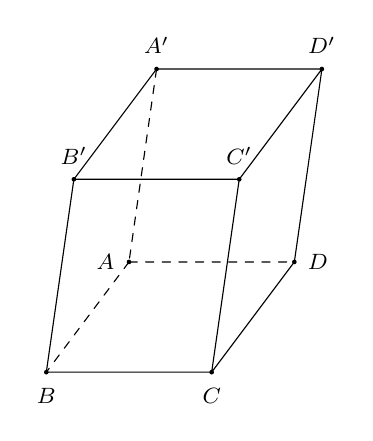
\begin{tikzpicture}[scale=0.7, font=\footnotesize, line join=round, line cap=round, >=stealth]
				\def\h{3.5}
				\def\dai{3}
				\def\x{0.5}
				\path (0,0)coordinate(A)
				--++(-1.5,-2) coordinate(B)
				--++(\dai,0) coordinate(C)
				(A)--+(\dai,0) coordinate (D)
				(A)--+(\x,\h) coordinate (A')
				(B)--+(\x,\h) coordinate (B')
				(C)--+(\x,\h) coordinate (C')
				(D)--+(\x,\h) coordinate (D')
				;
				\draw (B)--(C)--(D)  (A')--(B')--(C')--(D')--cycle (B)--(B') (C)--(C') (D)--(D');
				\draw[dashed] (A')--(A) (A)--(B) (A)--(D);
				\foreach \p/\q in {A/180,B/-90,C/-90,D/0,A'/90,B'/90,C'/90,D'/90}{
					\path (\p) node[shift={(\q:3mm)}]{$\p$};
					\fill[black] (\p) circle (1.2pt);}
		\end{tikzpicture}}
	}
\end{ex}
\Closesolutionfile{ans}

\ind{PHẦN II.} \inden{Câu trắc nghiệm đúng sai. Trong mỗi ý a), b), c), d) ở mỗi câu, học sinh chọn đúng hoặc sai.}\\
\setcounter{ex}{0}
\Opensolutionfile{ans}[ans/2D1-Bai1-DS]%--Đặt tên 2D1-Bai1-DS
\begin{ex}%[2H2H2-3]%[Dự án đề kiểm tra Toán 12 HKI NH24-25- Phạm Hoài]%[THPT Nguyễn Khuyến - An Giang]
	Cho hình hộp chữ nhật $OABC.O'A'B'C'$. Các vectơ đơn vị là $\overrightarrow{i}$, $\overrightarrow{j}$, $\overrightarrow{k}$ lần lượt trên các cạnh như hình vẽ. Biết $OA=3$, $OB=5$, $OO'=6$. Khi đó
	\begin{center}
			\begin{tikzpicture}[scale=0.6, font=\footnotesize,line join=round, line cap=round, >=stealth]
			\path
			(0,0) coordinate (O)
			++(-130:3) coordinate (A)
			++(0:4) coordinate (B)
			($(O)+(B)-(A)$) coordinate (C)
			;
			\foreach \i in {O,A,B,C}{
				\coordinate (\i') at ($(\i)+(0,4)$);
			}
			\draw (O')--(A')--(B')--(C')--cycle
			(A')--(A)--(B)--(B')  (B)--(C)--(C');
			\draw [red,->,thick](O)--++(-130:1)node[left]{$\overrightarrow {i}$};
			\draw [red,->,thick](O)--++(0:1)node[below]{$\overrightarrow {j}$};
			\draw [red,->,thick](O)--++(90:1)node[left]{$\overrightarrow {k}$};
			\draw [->,thick](A)--++(-130:1)node[right]{$x$};
			\draw [->,thick](C)--++(0:1)node[below]{$y$};
			\draw [->,thick](O')--++(90:1)node[left]{$z$};
			\draw[dashed,thin](O)--(A)(O)--(C)(O)--(O')
			[->](O)--(B')
			;
			\foreach \i/\g in {A'/90,B'/90,C'/90,O'/45,A/180,B/-90,C/-90,O/-90}
			\fill[black] (\i) circle(1pt)+(\g:5mm)node[scale=1]{$\i$};
		\end{tikzpicture}
	\end{center}
	\choiceTF
	{\True $\overrightarrow{OA}=3\overrightarrow{i}$}
	{$\overrightarrow{OO'}=5\overrightarrow{k}$}
	{$\overrightarrow{OC}=6\overrightarrow{j}$}
	{$\overrightarrow{OB'}=3\overrightarrow{i}+6\overrightarrow{j}+5\overrightarrow{k}$}
	\loigiai{
		\begin{itemchoice}
			\itemch $\overrightarrow{OA}=3\overrightarrow{i}$.
			\itemch $\overrightarrow{OO'}=6\overrightarrow{k}$.
			\itemch $\overrightarrow{OC}=5\overrightarrow{j}$.
			\itemch $\overrightarrow{OB'}=\overrightarrow{OA}+\overrightarrow{OC}+\overrightarrow{OO'}=3\overrightarrow{i}+5\overrightarrow{j}+6\overrightarrow{k}$.
		\end{itemchoice}
	}
\end{ex}
\begin{ex}%[2H2H2-3]%[Dự án đề cương 3 khối NH24-25 - Đợt 2 - Lê Phúc]
	Trong không gian $Oxyz$, cho vectơ $\overrightarrow{a}=2\overrightarrow{i}-3\overrightarrow{j}+4\overrightarrow{k}$.
	\choiceTF
	{\True Tọa độ của vectơ $\overrightarrow{a}$ là $\overrightarrow{a}=(2;-3;4)$}
	{Nếu $\overrightarrow{OA}=\overrightarrow{a}$ thì $A(-2;3;-4)$}
	{Nếu $\overrightarrow{c}=(3;0;1)$ thì $\overrightarrow{c}=3\overrightarrow{i}+\overrightarrow{j}$}
	{\True Biết $\overrightarrow{a}=\overrightarrow{b}$ và $\overrightarrow{b}=(3x-4;x-4y;4)$. Khi đó $x+y=2$}
	\loigiai{
		\begin{itemchoice}
			\itemch Tọa độ của vectơ $\overrightarrow{a}$ là $\overrightarrow{a}=(2;-3;4)$ 
			\itemch Nếu $\overrightarrow{OA}=\overrightarrow{a}$ thì $A(2;-3;4)$.
			\itemch Nếu $\overrightarrow{c}=(3;0;1)$ thì $\overrightarrow{c}=3\overrightarrow{i}+\overrightarrow{k}$.
			\itemch Ta có $\overrightarrow{a}=\overrightarrow{b}\Leftrightarrow \heva{&3x-y=2\\&x-4y=-3\\&4=4}\Leftrightarrow\ \heva{&x=1\\&y=1.}$\\
			Suy ra $x+y=2$.
		\end{itemchoice}
	}
\end{ex}

\begin{ex}%[2H2V2-3]%[Dự án đề cương 3 khối NH24-25 - Đợt 2 - Lê Phúc]
	Trong không gian $Oxyz$, cho 3 điểm $A(1; 0; 1)$, $B(2; 1; 2)$, $C(1;-1; 1)$.
	\choiceTF
	{\True $\overrightarrow{OA}=(1;0;1)$}
	{$\overrightarrow{OB}=(2;1;2)$}
	{\True $\overrightarrow{OC}=(1;-1;1)$}
	{Biết $\overrightarrow{OD}=\overrightarrow{OA}+\overrightarrow{OB}+\overrightarrow{OC}$. Tọa độ điểm $D$ là $(4;4;0)$}
	\loigiai{
		\begin{itemchoice}
			\itemch $\overrightarrow{OA}=(1;0;1)$.
			\itemch 
			$\overrightarrow{OB}=(2;1;2)$.
			\itemch 
			$\overrightarrow{OC}=(1;-1;1)$.
			\itemch 
		$\overrightarrow{OD}=\overrightarrow{OA}+\overrightarrow{OB}+\overrightarrow{OC}=\overrightarrow{i}+\overrightarrow{k}+2\overrightarrow{i}+\overrightarrow{j}+2\overrightarrow{k}+\overrightarrow{k}+\overrightarrow{i}-\overrightarrow{j}+\overrightarrow{k}=4\overrightarrow{i}+4\overrightarrow{k}$.\\
		Suy ra $\overrightarrow{OD}=(4;0;4)$ hay $D(4;0;4)$.
		\end{itemchoice}
	}
\end{ex}
%%%=============EX_3=============%%%
\begin{ex}%[2H2V2-6]%[Dự án đề cương 3 khối NH24-25 - Đợt 2 - Lê Phúc]
	Một máy bay đang cất cánh tại phi trường. Với hệ trục tọa độ $Oxyz$ được xác lập như hình bên. Cho biết $M$ là vị trí máy bay, $OM=14$, $\overrightarrow{NOB}=32^\circ$, $\overrightarrow{MOC}=65^\circ$. (\textit{Các kết quả làm tròn đến hàng phần chục})
	\begin{center}
			\begin{center}
			\begin{tikzpicture}[line join = round, line cap=round,>=stealth,font=\footnotesize,scale=1]
				\path 
				(0,0) coordinate (O)
				(-2,-2) coordinate (A')
				(4,0) coordinate (B')
				(0,3) coordinate (C')
				($(O)!0.3!(C')$) coordinate (C1)
				($(O)!0.3!(B')$) coordinate (B1)
				($(O)!0.3!(A')$) coordinate (A1)
				($(O)!0.8!(C')$) coordinate (C)
				($(O)!0.8!(B')$) coordinate (B)
				($(O)!0.8!(A')$) coordinate (A)
				;
				
				\foreach \diem/\t/\r in{A'/x/-90,
					B'/y/60,
					C'/z/60,
					A1/\overrightarrow{i}/-60,
					B1/\overrightarrow{j}/-90,
					C1/\overrightarrow{k}/180} 
				\draw[->,line width=1pt] (O)--(\diem)node[shift={(\r:4mm)},scale=1.2]{$\t$};
				
				\draw[dashed] 
				(A)--($(A)+(B)-(O)$) coordinate (N) --(B)
				(C)--($(C)+(N)-(O)$)coordinate (M) node[above=0.5cm]{$M$}--(N)
				(N)--(O)--(M);
				
				\draw (M);
				\draw pic[draw,angle radius=3mm] {right angle = O--A--N}; 
				\draw pic[draw,angle radius=3mm] {right angle = O--B--N}; 
				\draw pic[draw,angle radius=3mm] {right angle = O--C--M}; 
				\draw[cyan,line width=2pt,->] (O)--(M); 
				
				\foreach \p/\r in {A/160,B/90,C/180,N/-45,O/160}
				\fill (\p) circle (1.2pt) node[shift={(\r:3mm)}]{$\p$};
			\end{tikzpicture}
		\end{center}
	\end{center}
	\choiceTF
	{\True $OC=5{,}9$}
	{\True $ON=12{,}7$}
	{\True Điểm $N$ có tọa độ là $(10{,}8; 6{,}7; 0)$}
	{\True Điểm $M$ có tọa độ là $(6{,}7;10{,}8;5{,}9)$}
	\loigiai{
		\begin{itemchoice}
			\itemch Ta có $OC=14\cdot\cos65^\circ\approx 5{,}9$.
			\itemch Ta có $\overrightarrow{MOC}=\overrightarrow{OMN}=65^\circ$.\\ Suy ra $ON=14\cdot\sin65^\circ\approx 12{,}7$.
			\itemch \begin{itemize}
				\item $OA=ON\cdot\sin32^\circ=14\cdot\sin65^\circ\cdot\sin32^\circ\approx6{,}7$.
			\item $OA=ON\cdot\cos32^\circ=14\cdot\sin65^\circ\cdot\cos32^\circ\approx10{,}8$.
			\end{itemize}
		Suy ra $N(6{,7};10,8;0)$
			\itemch Ta có $M(6{,}7;10{,}8;5{,}9)$.
	\end{itemchoice}}
\end{ex}
\begin{ex}%[2H2V2-6]%[Dự án đề cương 3 khối NH24-25 - Đợt 2 - Lê Phúc]
	\immini{Cho hình hộp chữ nhật $OABC.O'A'B'C'$ có $OA=3$, $OD=4$, $OO'=5$. Chọn hệ trục tọa độ $Oxyz$ có gốc toạ độ $O$, các điểm $B$, $D$, $O'$ lần lượt thuộc các tia $Ox$, $Oy$, $Oz$.
	\choiceTF
	{\True $D(0;4;0)$}
	{\True $B(3;0;0)$}
	{$\overrightarrow{OB'}=3\overrightarrow{i}+5\overrightarrow{k}$}
	{\True Gọi $M$ là trung điểm của $OB'$. Ta có $M\left(\dfrac{3}{2};2;\dfrac{5}{2}\right)$}}
{	\begin{tikzpicture}[scale=0.6, font=\footnotesize,line join=round, line cap=round, >=stealth]
			\path
			(0,0) coordinate (O)
			++(-130:3) coordinate (A)
			++(0:4) coordinate (B)
			($(O)+(B)-(A)$) coordinate (C)
			;
			\foreach \i in {O,A,B,C}{
				\coordinate (\i') at ($(\i)+(0,4)$);
			}
			\draw (O')--(A')--(B')--(C')--cycle
			(A')--(A)--(B)--(B')  (B)--(C)--(C');
			\draw [red,->,thick](O)--++(-130:1)node[left]{$\overrightarrow {i}$};
			\draw [red,->,thick](O)--++(0:1)node[below]{$\overrightarrow {j}$};
			\draw [red,->,thick](O)--++(90:1)node[left]{$\overrightarrow {k}$};
			\draw [->,thick](A)--++(-130:1)node[right]{$x$};
			\draw [->,thick](C)--++(0:1)node[below]{$y$};
			\draw [->,thick](O')--++(90:1)node[left]{$z$};
			\draw[dashed,thin](O)--(A)(O)--(C)(O)--(O')
			[->](O)--(B')
			;
			\coordinate (M) at ($(O)!0.5!(B')$);
			\foreach \i/\g in {A'/90,B'/90,C'/90,O'/45,A/180,B/-90,C/-90,O/-90,M/90}
			\fill[black] (\i) circle(1pt)+(\g:5mm)node[scale=1]{$\i$};
		\end{tikzpicture}}
	\loigiai{
		\begin{itemchoice}
			\itemch Ta có $\overrightarrow{OB}=3\overrightarrow{i}$.\\
			Suy ra $\overrightarrow{OB}=(3;0;0)$ hay $B(3;0;0)$.
			\itemch Ta có $\overrightarrow{OD}=4\overrightarrow{j}$.\\
			Suy ra $\overrightarrow{OD}=(0;4;0)$ hay $D(0;4;0)$.
			\itemch Ta có $\overrightarrow{OB'}=\overrightarrow{OA}+\overrightarrow{OC}+\overrightarrow{OO'}=3\overrightarrow{i}+4\overrightarrow{j}+5\overrightarrow{k}$.
			\itemch $\overrightarrow{OM}=\dfrac{1}{2}\overrightarrow{OB'}=\dfrac{3}{2}\overrightarrow{i}+2\overrightarrow{j}+\dfrac{5}{2}\overrightarrow{k}$.\\
			Suy ra $\overrightarrow{OM}=\left(\dfrac{3}{2};2;\dfrac{5}{2}\right)$ hay $M\left(\dfrac{3}{2};2;\dfrac{5}{2}\right)$.
		\end{itemchoice}
	}
\end{ex}
\Closesolutionfile{ans}


\ind{PHẦN III.} \inden{Câu trả lời ngắn}\\
\setcounter{ex}{0}
\Opensolutionfile{ans}[ans/2D1-Bai1-DS]%--Đặt tên 2D1-Bai1-DS
\begin{ex}%[2H2H2-2]%[Dự án đề cương 3 khối NH24-25 - Đợt 2 - Lê Phúc]
	Trong không gian $Oxyz$ cho $\overrightarrow{OM}=3\overrightarrow{i}+7\overrightarrow{j}-5\overrightarrow{k}$. Khi đó cao độ của điểm $M$ bằng
	\shortans{$-5$}
	\loigiai{
	$\overrightarrow{OM}=3\overrightarrow{i}+7\overrightarrow{j}-5\overrightarrow{k}\Rightarrow \overrightarrow{OM}=(3;7;-5)$.\\
	Suy ra $M(3;7;-5)$.\\
	Vậy cao độ của điểm $M$ là $-5$.
	}
\end{ex}
\begin{ex}%[2H2H2-2]%[Dự án đề cương 3 khối NH24-25 - Đợt 2 - Lê Phúc]
	Trong không gian $Oxyz$ cho $\overrightarrow{a}=(3;-2;1)$ và $\overrightarrow{b}=(3;m+2;1)$. Tìm $m$ sao cho $\overrightarrow{a}=\overrightarrow{b}$.
	\shortans{$-4$}
	\loigiai{
	Để $\overrightarrow{a}=\overrightarrow{b}$ thì 
	\[-2=m+2\Leftrightarrow m=-4.\]
	}
\end{ex}
\begin{ex}%[2H2V2-2]%[Dự án đề cương 3 khối NH24-25 - Đợt 2 - Lê Phúc]
	Trong không gian $Oxyz$ cho $\overrightarrow{u}=(1;2;-1)$. Biết $\overrightarrow{u}=x\overrightarrow{i}+y\overrightarrow{j}+z\overrightarrow{k}$, với $x$, $y$, $z\in \mathbb{R}$. Tính $x+y+z$.
	\shortans{$2$}
	\loigiai{
	Ta có $\overrightarrow{u}=(1;2;-1)$.\\
	Suy ra $\overrightarrow{u}=\overrightarrow{i}+2\overrightarrow{j}-\overrightarrow{k}$.\\
	Do đó $\heva{&x=1\\&y=2\\&z=-1}$.\\
	Vậy $x+y+z=1+2-1=2$.}
\end{ex}
\begin{ex}%[2H2H2-2]%[Dự án đề cương 3 khối NH24-25 - Đợt 2 - Lê Phúc]
	\immini[thm]{
		Để chuẩn bị cho ngày hội thao, người ta dựng bốn chiếc cột tại bốn góc của một sân bóng hình chữ nhật với kích thước là $15\ \mathrm{m} \times 25\ \mathrm{m}$. Bốn chiếc cột vuông góc với mặt sân và có chiều cao lần lượt là $3$ mét, $4$ mét, $6$ mét và $c$ mét. Một tấm bạt lớn được căng phẳng với bốn góc được cố định vào đầu bốn cột. Xét hệ trục tọa độ $Oxyz$ như hình vẽ bên (đơn vị trên các trục là mét) thì điểm $C$ có tọa độ là $(a; b; c)$. Tính $a-2b+c$.
		\shortans[]{$-35$}	
	}{
		\begin{tikzpicture}[>=stealth,line join=round,line cap=round,font=\footnotesize,scale=1]
			%	\def\cao{3};
			\path
			(0,0) coordinate (A)
			(0:5) coordinate (D)
			(90:0.6) coordinate (A')
			(-120:3) coordinate (B)
			($(B)+(D)-(A)$) coordinate (C)
			($(B)+(90:0.8)$) coordinate (B')
			($(C)+(90:1.2)$) coordinate (C')
			($(D)+(90:1.2)$) coordinate (D')
			(-120:4) coordinate (x)
			(6,0) coordinate (y)
			(0,2) coordinate (z)
			;
			\draw[->] (D)--(y)node[below right]{$y$};
			\draw[->] (B)--(x)node[below right]{$x$};
			\draw[->] (A')--(z)node[below right]{$z$};
			\draw
			(A')--(B')--(C')--(D')--cycle (B')--(B)node[midway,left]{\scriptsize 4m}--(C)node[midway,below]{\scriptsize 25m}--(C')node[midway,left]{\scriptsize 6m} (C)--(D)node[midway,right]{\scriptsize 15m}--(D')node[midway,right]{\scriptsize $c$}
			;
			\node at ($(A)+(-35:0.5)$){\scriptsize $O \equiv A$};
			\draw[dashed] (A')--(A)node[midway,right]{\scriptsize 3m}--(B) (A)--(D);
			\foreach \x/\g in {B/180,C/-45,D/45,A'/180,B'/135,C'/0,D'/45}\fill[black](\x) circle (1pt) +(\g:3mm) node {$\x$};
		\end{tikzpicture}
	}
	\loigiai{
	Ta có $\overrightarrow{OC}=\overrightarrow{OB}+\overrightarrow{OD}=15\overrightarrow{i}+25\overrightarrow{j}$.\\
	Suy ra $\overrightarrow{OC}=(15;25;0)$ hay $C(15;25;0)$.\\
	Vậy $a-2b+c=15-2\cdot25+0=-35$.
	}
\end{ex}

\begin{ex}%[2H2H2-2]%[Dự án đề cương 3 khối NH24-25 - Đợt 2 - Lê Phúc]
	Một phòng khách có thiết kế dạng hình hộp chữ nhật với chiều dài là $6$ m, chiều rộng là $4$ m và chiều cao là $4$ m. Một quạt trần được treo tại chính giữa trần nhà của phòng khách. Xét hệ trục tọa độ $Oxyz$ có gốc $O$ trùng với một góc phòng và mặt phẳng $(Oxy)$ trùng với mặt sàn, đơn vị đo được lấy theo mét (Hình vẽ).
	\begin{center}
		\begin{tikzpicture}[scale=.7, font=\footnotesize, line join=round, line cap=round, >=stealth]
			\path 
			(0:0) coordinate (A)
			($(A)+(-135:1)$) coordinate (x)
			(0:4.5) coordinate (B)
			($(A)+(45:2)$) coordinate (O)
			($(O)+(B)-(A)$) coordinate (C)
			($(C)+(0:1)$) coordinate (y)
			($(O)+(90:3)$) coordinate (O')
			($(O')+(90:1)$) coordinate (z)
			($(A)+(90:3)$) coordinate (A')
			($(B)+(90:3)$) coordinate (B')
			($(C)+(90:3)$) coordinate (C')
			($(O)!1/3!(A)$) coordinate (a)
			($(O)!1/3!(O')$) coordinate (o')
			($(O)!1/5!(C)$) coordinate (c)
			;
			\draw[->] (O')--(z) node[left]{$z$};
			\draw[->] (C)--(y) node[below]{$y$};
			\draw[->] (A)--(x) node[right]{$x$};
			\draw 	(O')--(A')--(B')--(C')--cycle
			(A')--(A)--(B)--(C) (B')--(B) (C')--(C)
			pic[draw,angle radius=2mm]{right angle=C--O--O'}
			pic[draw,angle radius=2mm]{right angle=A--O--C}
			pic[draw,angle radius=2mm]{right angle=O'--O--A}
			;
			\draw[dashed] (A)--(O) (O)--(C) (O)--(O');
			\foreach \x/\g in {O/180}
			\draw[fill=black] 	(\x) circle (.5pt)	($(\g:.5)+(\x)$) node {$\x$};	
		\end{tikzpicture}
	\end{center}
	Biết vị trí treo quạt trần là điểm $M(a;b;c)$. Tính $S=a+b+c$.
	\shortans{$7$}
	\loigiai{
		\begin{center}
			\begin{tikzpicture}[scale=.7, font=\footnotesize, line join=round, line cap=round, >=stealth]
				\path 
				(0:0) coordinate (A)
				($(A)+(-135:1)$) coordinate (x)
				(0:4.5) coordinate (B)
				($(A)+(45:2)$) coordinate (O)
				($(O)+(B)-(A)$) coordinate (C)
				($(C)+(0:1)$) coordinate (y)
				($(O)+(90:3)$) coordinate (O')
				($(O')+(90:1)$) coordinate (z)
				($(A)+(90:3)$) coordinate (A')
				($(B)+(90:3)$) coordinate (B')
				($(C)+(90:3)$) coordinate (C')
				($(O)!1/3!(A)$) coordinate (a)
				($(O)!1/3!(O')$) coordinate (o')
				($(O)!1/5!(C)$) coordinate (c)
				;
				\coordinate (M) at ($(O')!0.5!(B')$);
				\draw[dashed] (A)--(O) (O)--(C) (O)--(O') (O)--(B') (O)--(M);
				\draw[->] (O')--(z) node[left]{$z$};
				\draw[->] (C)--(y) node[below]{$y$};
				\draw[->] (A)--(x) node[right]{$x$};
				\draw 	(O')--(A')--(B')--(C')--cycle
				(A')--(A)--(B)--(C) (B')--(B) (C')--(C) (O')--(B')
				pic[draw,angle radius=2mm]{right angle=C--O--O'}
				pic[draw,angle radius=2mm]{right angle=A--O--C}
				pic[draw,angle radius=2mm]{right angle=O'--O--A}
				;
				\foreach \x/\g in {A/170,B/-15,C/-30,O/180,A'/170,B'/-15,C'/0,O'/180,M/90}
				\draw[fill=black] 	(\x) circle (1pt)	($(\g:.5)+(\x)$) node {$\x$};	
			\end{tikzpicture}
		\end{center}
	Ta có
	\begin{eqnarray*}
	\overrightarrow{OM}&=&\dfrac{1}{2}\left(\overrightarrow{OB'}+\overrightarrow{OO'}\right)\\
	&=&\dfrac{1}{2}\left(\overrightarrow{OA}+\overrightarrow{OC}+2\overrightarrow{OO'}\right)\\
	&=&\dfrac{1}{2}\left(4\overrightarrow{i}+6\overrightarrow{j}+4\overrightarrow{k}\right)\\
	&=&2\overrightarrow{i}+3\overrightarrow{j}+2\overrightarrow{k}.
	\end{eqnarray*} 
	Suy ra $\overrightarrow{OM}=(2;3;2)$ hay $M(2;3;2)$.\\
	Vậy $S=a+b+c=7$
	}
\end{ex}
\Closesolutionfile{ans}


\ind{PHẦN IV.} \inden{Tự luận.}\\
\setcounter{ex}{0}
\begin{ex}%[2H2N2-3]%[Dự án đề cương 3 khối NH24-25 - Đợt 2 - Lê Phúc]
Trong không gian $Oxyz$ biết
\begin{enumerate}
	\item $\overrightarrow{u}=2\overrightarrow{i}-3\overrightarrow{j}$, $\overrightarrow{v}=-\overrightarrow{k}+\overrightarrow{u}+3\overrightarrow{j}$. Tìm tọa độ các vectơ $\overrightarrow{u}$ và $\overrightarrow{v}$.
	\item $\overrightarrow{OI}=\overrightarrow{i}+\overrightarrow{j}+\overrightarrow{k}$, $\overrightarrow{OJ}=\overrightarrow{OI}-2\overrightarrow{i}+\overrightarrow{k}$. Tìm tọa độ điểm $I$ và $J$.
\end{enumerate}
\loigiai{
	\begin{enumerate}
	\item	\begin{itemize}
		\item $\overrightarrow{u}=2\overrightarrow{i}-3\overrightarrow{j}=(2;-3;0)$.
		\item $\overrightarrow{v}=-\overrightarrow{k}+\overrightarrow{u}+3\overrightarrow{j}=-\overrightarrow{k}+2\overrightarrow{i}=(2;0;-1)$.
		\end{itemize}
	\item \begin{itemize}
		\item $\overrightarrow{OI}=\overrightarrow{i}+\overrightarrow{j}+\overrightarrow{k}=(1;1;1)$.\\
		Suy ra $I(1;1;1)$.
		\item $\overrightarrow{OJ}=\overrightarrow{OI}-2\overrightarrow{i}+\overrightarrow{k}=\overrightarrow{i}+\overrightarrow{j}+\overrightarrow{k}-2\overrightarrow{i}+\overrightarrow{k}=-\overrightarrow{i}+\overrightarrow{j}+2\overrightarrow{k}=(-1;1;2)$.\\
		Suy ra $J(-1;1;2)$.
	\end{itemize}
\end{enumerate}}
\end{ex}
\begin{ex}%[2H2N2-2]%[Dự án đề cương 3 khối NH24-25 - Đợt 2 - Lê Phúc]
	Trong không gian $Oxyz$, cho ba vectơ $\overrightarrow{a}=(1;0;1),\overrightarrow{b}=(1;1;0)$ và $\overrightarrow{d}=2\overrightarrow{a}+3\overrightarrow{b}$. Tìm tọa độ của $\overrightarrow{d}$.
	\loigiai{
		Ta có $\overrightarrow{d}=2\overrightarrow{a}+3\overrightarrow{b}=2\left(\overrightarrow{i}+\overrightarrow{k}\right)+3\left(\overrightarrow{i}+\overrightarrow{j}\right)=5\overrightarrow{i}+2\overrightarrow{j}+3\overrightarrow{k}$.\\
		Suy ra $\overrightarrow{d}=(5;2;3)$.
	}	
\end{ex}
\begin{ex}%[2H2N2-2]%[Dự án đề cương 3 khối NH24-25 - Đợt 2 - Lê Phúc]
	Trong không gian $O x y z$, cho $\overrightarrow{OM}=\overrightarrow{i}+a \cdot \overrightarrow{j}+b \cdot \overrightarrow{k}(a, b \in \mathbb{R} )$. Tọa độ của điểm $M$ là
	\loigiai{
		Do $\overrightarrow{OM}=\overrightarrow{i}+a \cdot \overrightarrow{j}+b \cdot \overrightarrow{k}$ nên tọa độ của điểm $M(1 ; a ; b)$.}
\end{ex}
\begin{ex}%[2H2H2-2]%[Dự án đề cương 3 khối NH24-25 - Đợt 2 - Lê Phúc]
	Trong không gian $Oxyz$, cho hai điểm $A(1 ; 1 ;-2)$ và $B(2 ; 2 ; 1)$. Vectơ $\overrightarrow{A B}$ có tọa độ là
		\loigiai{
		$\overrightarrow{AB}=\overrightarrow{OB}-\overrightarrow{OA}=2\overrightarrow{i}+2\overrightarrow{j}+\overrightarrow{k}-\overrightarrow{i}-\overrightarrow{j}+2\overrightarrow{k}=\overrightarrow{i}+\overrightarrow{j}+3\overrightarrow{k}$.\\
		Suy ra $\overrightarrow{AB}=(1;1;3)$.}
\end{ex}
\begin{ex}%[2H2N2-2]%[Dự án đề cương 3 khối NH24-25 - Đợt 2 - Lê Phúc]
	\immini{
		Cho hình chóp $S.ABCD$ có đáy là hình vuông cạnh bằng $1$, $SA=2$ và \\$SA \perp(ABCD)$. Chọn hệ trục $Oxyz$ có gốc tọa độ tại $A$; các điểm $B$, $D$, $S$ lần lượt trên các tia $Ox$, $Oy$, $Oz$. Tìm tọa độ của các điểm $S$, $C$.
	}
	{
		\begin{tikzpicture}[declare function={a=2.65;b=4.5;h=3;},line join=round,line cap=round,font=\footnotesize,>=stealth,scale=0.6]
			\path (0,0) coordinate (A)
			(-135:a) coordinate (B)
			(b,0) coordinate (D)
			($(D)-(A)+(B)$) coordinate (C)
			(0,h) coordinate (S)
			($(B)!-0.3!(A)$) coordinate (x)
			($(D)!-0.3!(A)$) coordinate (y)
			($(S)!-0.3!(A)$) coordinate (z)
			($(B)!.5!(C)$)  coordinate (E)
			;
			\draw[dashed] (S)--(A)--(B) (A)--(D);
			\draw (B)--(C)--(D) (B)--(S)  (D)--(S)--(C) ;
			\draw [->] (B)--(x)node[below]{$x$} ;
			\draw [->]  (D)--(y)node[right]{$y$};
			\draw [->]  (S)--(z)node[above]{$z$};
			\foreach \t/\g in {A/180,B/-90,C/-90,D/-60,S/120}{
				\draw[fill=black] (\t) circle (1pt) node[shift={(\g:7pt)},font=\scriptsize]{$ \t $};
			}
		\end{tikzpicture}
	} 
	\loigiai{
		\begin{itemize}
			\item $\overrightarrow{AS}=2\overrightarrow{k}$.\\
			Suy ra $\overrightarrow{AS}=(0;0;2)$ hay $S(0;0;2)$.
			\item $\overrightarrow{AC}=\overrightarrow{AB}+\overrightarrow{AD}=\overrightarrow{i}+\overrightarrow{j}$.\\
			Suy ra $\overrightarrow{AC}=(1;1;0)$ hay $C(1;1;0)$.
		\end{itemize}
	}
\end{ex}
\begin{ex}%[2H2H2-2]%[Dự án đề cương 3 khối NH24-25 - Đợt 2 - Lê Phúc]
	Trong không gian $Oxyz$ cho hình hộp chữ nhật $ABCD.A'B'C'D'$ với $A\equiv O$, $B\in$ tia $Ox$, $D\in$ tia $Oy$, $A'\in$ tia $Oz$. Biết $AB=2$, $AD=4$, $AA'=5$  và tọa độ điểm $C'(a;b;c)$. Tính tổng $a+b+c$.
	\loigiai{
\immini{	Ta có $\overrightarrow{AC'}=\overrightarrow{AB}+\overrightarrow{AD}+\overrightarrow{AA'}=2\overrightarrow{i}+4\overrightarrow{j}+5\overrightarrow{k}$.\\
	Suy ra $\overrightarrow{AC'}=(2;4;5)$ hay $C'(2;4;5)$.\\
	Vậy $a+b+c=2+4+5=11$.}
	{\begin{tikzpicture}[scale=0.6, font=\footnotesize,line join=round, line cap=round, >=stealth]
			\path
			(0,0) coordinate (A)
			++(-130:3) coordinate (B)
			++(0:4) coordinate (C)
			($(A)+(C)-(B)$) coordinate (D)
			;
			\foreach \i in {A,B,C,D}{
				\coordinate (\i') at ($(\i)+(0,4)$);
			}
			\draw (A')--(B')--(C')--(D')--cycle
			(B')--(B)--(C)--(C')  (C)--(D)--(D');
			\draw [red,->,thick](A)--++(-130:1)node[left]{$\overrightarrow {i}$};
			\draw [red,->,thick](A)--++(0:1)node[below]{$\overrightarrow {j}$};
			\draw [red,->,thick](A)--++(90:1)node[left]{$\overrightarrow {k}$};
			\draw [->,thick](B)--++(-130:1)node[right]{$x$};
			\draw [->,thick](D)--++(0:1)node[below]{$y$};
			\draw [->,thick](A')--++(90:1)node[left]{$z$};
			\draw[dashed,thin](A)--(B)(A)--(D)(A)--(A')
			[->](A)--(C')
			;
			\foreach \i/\g in {A'/45,B'/90,C'/-30,D'/45,A/180,B/180,C/-90,D/-90}
			\fill[black] (\i) circle(1pt)+(\g:5mm)node[scale=1]{$\i$};
		\end{tikzpicture}}

	}
\end{ex}

\begin{ex}%[2H2H2-6]%[Dự án đề cương 3 khối NH24-25 - Đợt 2 - Lê Phúc]
	(\textit{Trích đề thi CKI - Trường THPT Nguyễn Du - Năm học 2024-2025})\\
	Một chiếc xe đang kéo căng sợi dây cáp $AB$ trong công trường xây dựng, trên đó đã thiết lập hệ toạ độ $Oxyz$ như hình vẽ với độ dài đơn vị trên trục toạ độ bằng 1 mét. Ta tìm được toạ độ của véc-tơ $\overrightarrow{AB}=(a;b;c)$. Tính $a+b+c$. (\textit{kết quả viết dưới dạng số thập phân và làm tròn đến hàng phần chục}). 
	\loigiai{
		\begin{center}
			\begin{tikzpicture}[line join = round, line cap=round,>=stealth,font=\footnotesize,scale=0.75]
				\path (0,0) coordinate (O)
				(5,0)	coordinate (H)
				(-2,-2)	coordinate (K)
				($(K)+(H)-(O)$) coordinate (B)
				($(O)+(0,3.6)$) coordinate (A)
				;
				\foreach \x/\y in{K/x,H/y,A/z}
				\draw[->,line width=1pt,scale=1.5] (O)--(\x)--($(O)!1.4!(\x)$)node[right]{$\y$};
				\draw[pattern=crosshatch]   (-0.2,0) rectangle (0.3,4)
				(-2.5,3.6) rectangle (0.3,4);
				\draw[pattern=crosshatch,rotate=-50,xshift=-3cm,yshift=2.4cm]  
				(-0.2,0) rectangle (0.3,1.5);
				\draw[cyan,line width=4pt] (O)--(A);
				\foreach \p/\r in {A/0,K/180,H/90,B/70,O/-90}
				\fill (\p) circle (1.2pt) node[shift={(\r:3.5mm)}]{$\p$};
				\draw[dashed] (O)--($(O)-(1,0)$);
				\draw[<->,line width=2pt] ($(O)-(1,0)$)--($(A)-(1,0)$)node[pos=0.5,left,scale=2]{$10$ m};
				\draw[line width=1pt] (O)--(B) node[pos=0.45,below,scale=1.5,rotate=-30]{$15$ m};
				\draw (K)--(B)--(H) (B)--(O);
				\draw pic[draw,angle radius=6mm] {angle = B--O--H};
				\draw ($(O)+(1.2,-0.25)$)  node{$30^\circ$};
				\draw[->,line width=2pt] (A)--(B);
				\draw (B) node[xshift=0.5cm,yshift=-0.5cm]{
					\begin{tikzpicture}[line join = round, line cap=round,>=stealth,font=\footnotesize,scale=0.4]
						\draw[rotate=-65,scale=1,line width=5pt,xshift=1.8cm,yshift=2.4cm] (0.7,-1.5)  ellipse (0.4cm and 0.3cm);
						\fill[green!80] (0,0)--(0,-1)--(1,-2)--(2,-2)--(2,-1)--(1,0)--cycle;
						\draw (0,0)--(0,-1)--(1,-2)--(2,-2)--(2,-1)--(1,0)--cycle;
						\draw[rotate=-65,scale=1,line width=5pt] (1,-0.4)  ellipse (0.4cm and 0.3cm);
						\draw[rotate=-65,scale=1,,line width=5pt,xshift=1.4cm,yshift=1.5cm] (0.7,-1.5)  ellipse (0.4cm and 0.3cm);
					\end{tikzpicture}	
				};
			\end{tikzpicture}
		\end{center}
		$\overrightarrow{AB}=\overrightarrow{OB}-\overrightarrow{OA}=\overrightarrow{OK}+\overrightarrow{OH}-\overrightarrow{OA}$.\\
		$OH=OB\cdot\cos 30^\circ =\dfrac{15\sqrt{3}}{2}$ và $OK=OB\cdot\cos 60^\circ =\dfrac{15}{2}$. \\
		Suy ra $\overrightarrow{AB}=\dfrac{15}{2}\overrightarrow{i}+\dfrac{15\sqrt{3}}{2}\overrightarrow{j}-10\overrightarrow{j}$.\\
		Do đó $\overrightarrow{AB}=\left(\dfrac{15}{2};\dfrac{15\sqrt{3}}{2};-10\right)$.\\
		Vậy $a+b+c=\dfrac{15}{2}+\dfrac{15\sqrt{3}}{2}+(-10)\approx10{,}5$.
	} 
\end{ex}
\begin{ex}%[2H2V2-6]%[Dự án đề cương 3 khối NH24-25 - Đợt 2 - Lê Phúc]
	(\textit{Trích đề thi CKI - Trường THPT Phan Ngọc Hiền - Năm học 2024-2025})\\
	\immini{
		Một phòng học có thiết kế dạng hình hộp chữ nhật với chiều dài là $8$ m, chiều rộng là $6$ m và chiều cao là $3$ m. Một chiếc đèn được treo tại chính giữa trần nhà của phòng học. Xét hệ trục tọa độ $Oxyz$ có gốc $O$ trùng với một góc phòng và mặt phẳng $(Oxy)$ trùng với mặt sàn, đơn vị đo được lấy theo mét. Tọa độ điểm treo đèn là $I(a;b;c)$. Tính tổng $a+b+c$.
	}{
		\begin{tikzpicture}[font=\footnotesize, line join=round, line cap=round, >=stealth, scale=0.6]
			\def\r{-140}
			\def\c{3}
			\def\d{4}
			\path
			(0:0) coordinate (O)++(0:\c+3)
			coordinate (D)++(90:\c)coordinate(D')
			(O)++(\r:\d) coordinate (B)++(0:\c+3) coordinate (C)++(90:\c)coordinate(C')
			(O)++(90:\c) coordinate (A')++(\r:\d) coordinate (B')
			($(O)!1.4!(B)$) coordinate (x)
			($(O)!1.3!(D)$) coordinate (y)
			($(O)!1.4!(A')$) coordinate (z)
			;
			\draw (A')--(B')--(B)--(C)--(D)--(D')--(A') (C)--(C') (B')--(C')--(D');
			\draw[dashed] (A')--(O)--(B) (O)--(D);
			\foreach \p / \r in {B/x,D/y,A'/z}
			\draw[->] (\p)--(\r);
			\foreach \p / \r in {O/180}
			\fill (\p) circle (1.2pt) node[shift={(\r:3mm)}]{$\p$};
			\node at ($(O)!0.7!(A')$) [right] {$3$ m};
			\node at ($(O)!0.3!(D)$) [below] {$8$ m};
			\node at ($(O)!0.5!(B)$) [right] {$6$ m};
			\foreach \p / \r in {x/-135,y/45,z/30}
			\fill (\p) node[shift={(\r:3mm)}]{$\p$};
		\end{tikzpicture}
	}
	\loigiai{
		\immini{
		Giả sử hình hộp chữ nhật là $OBCD.O'B'C'D'$.\\
			Ta có
		\begin{eqnarray*}
			\overrightarrow{OI}&=&\dfrac{1}{2}\left(\overrightarrow{OO'}+\overrightarrow{OC'}\right)\\
			&=&\dfrac{1}{2}\left(\overrightarrow{OO'}+\overrightarrow{OO'}+\overrightarrow{OB}+\overrightarrow{OD}\right)\\
			&=&\dfrac{1}{2}\left(6\overrightarrow{k}+6\overrightarrow{i}+8\overrightarrow{j}\right)\\
			&=&3\overrightarrow{k}+3\overrightarrow{i}+4\overrightarrow{j}.
		\end{eqnarray*}
		Suy ra $\overrightarrow{OI}=(3;4;3)$.\\
		Do đó $I(3;4;3)$.\\
		Vậy $a+b+c=3+4+3=10$.
		}{
			\begin{tikzpicture}[font=\footnotesize, line join=round, line cap=round, >=stealth, scale=0.6]
				\def\r{-140}
				\def\c{3}
				\def\d{4}
				\path
				(0:0) coordinate (O)++(0:\c+3)
				coordinate (D)++(90:\c)coordinate(D')
				(O)++(\r:\d) coordinate (B)++(0:\c+3) coordinate (C)++(90:\c)coordinate(C')
				(O)++(90:\c) coordinate (O')++(\r:\d) coordinate (B')
				($(O)!1.4!(B)$) coordinate (x)
				($(O)!1.3!(D)$) coordinate (y)
				($(O)!1.4!(O')$) coordinate (z)
				;
				\draw (O')--(B')--(B)--(C)--(D)--(D')--(O') (C)--(C') (B')--(C')--(D') (O')--(C');
				\draw[dashed] (A')--(O)--(B) (O)--(D) (O)--(I) (O)--(C');
				\coordinate (I) at ($(O')!1/2!(C')$);
				\foreach \p / \r in {B/x,D/y,O'/z}
				\draw[->] (\p)--(\r);
				\foreach \p / \r in {O/180,I/45,O'/45,C'/90,B'/180,D'/90,B/-90,C/-90,D/45}
				\fill (\p) circle (1.2pt) node[shift={(\r:3mm)}]{$\p$};
				\node at ($(O)!0.5!(O')$) [left] {$3$ m};
				\node at ($(O)!0.3!(D)$) [below] {$8$ m};
				\node at ($(O)!0.5!(B)$) [right] {$6$ m};
				\foreach \p / \r in {x/-135,y/45,z/30}
				\fill (\p) node[shift={(\r:3mm)}]{$\p$};
			\end{tikzpicture}
		}
}
\end{ex}
\begin{ex}%[2H2V2-6]%[Dự án đề cương 3 khối NH24-25 - Đợt 2 - Lê Phúc]
		(\textit{Trích đề thi CKI - Trường THPT Bình Chiểu - Năm học 2024-2025})\\
	Một chú chim bồ câu đang ở vị trí $M$ trong không gian $Oxyz$ như hình sau. Gọi $H$ là hình chiếu vuông goác của $M$ xuống mặt phẳng $(Oxy)$. Biết $OM=100$, $(\vec{i},\overrightarrow{OH})=60^{\circ}$, $(\overrightarrow{OH},\overrightarrow{OM})=45^{\circ}$. Khi đó tọa độ của điểm $M$ là $M(a;b;c)$. 
\begin{center}
	\begin{tikzpicture}[scale=0.75, font=\footnotesize,>=stealth]
		\path
		(0,0) coordinate (O)
		(-2,-2) coordinate (A)
		(3,-2) coordinate (H)
		(5,0) coordinate (B)
		(3,1) coordinate (M)
		(0,3) coordinate (C)
		;
		\draw[->] (0,0)--(6,0) node[below]{$y$};
		\draw[->] (0,0)--(-3,-3) node[below]{$x$};
		\draw[->] (0,0)--(0,4) node[left]{$z$};
		\draw[dashed] (C)--(M)--(H)--(A) (O)--(H)--(B);
		\draw[fill=blue] (M)circle (0.15)--(O)node[midway,sloped,scale=1,above]{$100$};
		\foreach \x/\g in {O/160,H/-90,M/30,A/-80,B/-70,C/30}\draw[fill=black] (\x) circle (.05) +(\g:.5)node{\footnotesize$\x$};
		\foreach \x/\y/\z in {H/A/O,H/B/O,M/C/O}{\path pic[draw,angle radius=5pt]{right angle= \x--\y--\z};}
		\draw pic["\scriptsize$45^\circ$",draw,angle eccentricity=1.9,angle radius=0.45cm]{angle=H--O--M};
		\draw pic["\scriptsize$60^\circ$",draw,angle eccentricity=1.9,angle radius=0.3cm]{angle=A--O--H};
	\end{tikzpicture}
\end{center}
Tính giá trị biểu thức $S=a-b+c$ (làm tròn tới hàng đơn vị).
\shortans{$50$}
\loigiai{
	Tam giác $OMH$ vuông tại $H$, $OM = 100$; $\widehat{MOH} = 45^\circ$ nên ta có 
	\begin{itemize}
		\item [$\bullet$] $OH = OM\cdot \cos 45=100\cdot\dfrac{\sqrt{2}}{2} \approx 70{,}7$
		\item [$\bullet$] $OC = MH = OM \cdot \sin 45 \approx 70{,}7$.
	\end{itemize}
	Tam giác $OAH$ vuông tại $A$, $OH = 70{,}7$; $\widehat{AOH} = 60^\circ$ nên ta có 
	\begin{itemize}
		\item [$\bullet$] $OA = OH\cdot \cos 60 \approx 35{,}4$,
		\item [$\bullet$] $OB = AH = OH\cdot \sin 60 \approx 61{,}2$.
	\end{itemize}
	Suy ra 
	\begin{eqnarray*}
		\overrightarrow{OM} & = & \overrightarrow{OC} + \overrightarrow{OH} = \overrightarrow{OC} + \overrightarrow{OA}+\overrightarrow{OB} \\
		& = & 35{,}4\overrightarrow{i}+61{,}2\overrightarrow{j}+70{,}7\overrightarrow{k}.
	\end{eqnarray*}
	Vậy $M(35{,}4; 61{,}2; 70{,}7)$. \\
	Khi đó $a-b+c=35{,}4-61{,}2+70{,}7\approx 50$
}
\end{ex}
\begin{ex}%[2H2V2-6]%[Dự án đề cương 3 khối NH24-25 - Đợt 2 - Lê Phúc]
	Ở một sân bay, vị trí của máy bay được xác định bởi điểm $P$ trong không gian $Oxyz$ (như hình vẽ).
	Gọi $H$ là hình chiếu vuông góc của $M(a;b;c)$ xuống mặt phẳng $(Oxy)$. Cho biết $OM=79$, $\left(\overrightarrow{i},\overrightarrow{OH}\right)=68^{\circ}$, $\left(\overrightarrow{OH},\overrightarrow{OM}\right)=50^{\circ}$. Tính giá trị của biểu thức $S=a+b+c$ (\textit{kết quả làm tròn đến hàng đơn vị}).
	\begin{center}
		\begin{tikzpicture}[line join = round, line cap=round,>=stealth,font=\footnotesize,scale=1]
			\path 
			(0,0) coordinate (O)
			(-2,-2) coordinate (A')
			(4,0) coordinate (B')
			(0,3) coordinate (C')
			($(O)!0.3!(C')$) coordinate (C1)
			($(O)!0.3!(B')$) coordinate (B1)
			($(O)!0.3!(A')$) coordinate (A1)
			($(O)!0.8!(C')$) coordinate (C)
			($(O)!0.8!(B')$) coordinate (B)
			($(O)!0.8!(A')$) coordinate (A)
			;
			
			\foreach \diem/\t/\r in{A'/x/-90,
				B'/y/60,
				C'/z/60,
				A1/\overrightarrow{i}/-60,
				B1/\overrightarrow{j}/-90,
				C1/\overrightarrow{k}/180} 
			\draw[->,line width=1pt] (O)--(\diem)node[shift={(\r:4mm)},scale=1.2]{$\t$};
			
			\draw[dashed] 
			(A)--($(A)+(B)-(O)$) coordinate (H) --(B)
			(C)--($(C)+(H)-(O)$)coordinate (M) node[above=0.5cm]{$M$}--(H)
			(H)--(O)--(M);
			
			\draw (M);
			\draw pic[draw,angle radius=3mm] {right angle = O--A--H}; 
			\draw pic[draw,angle radius=3mm] {right angle = O--B--H}; 
			\draw pic[draw,angle radius=3mm] {right angle = O--C--M}; 
			\draw[cyan,line width=2pt,->] (O)--(M); 
			
			\foreach \p/\r in {A/160,B/90,C/180,H/-45,O/160}
			\fill (\p) circle (1.2pt) node[shift={(\r:3mm)}]{$\p$};
		\end{tikzpicture}
	\end{center}
	\loigiai{
		Ta có $OC=MH=OM \cdot \sin \left(\overrightarrow{OH}, \overrightarrow{OM}\right)=79\cdot \sin 50^{\circ} \approx 60{,}52$.\\
		$OH=OM \cdot \cos \left(\overrightarrow{OH}, \overrightarrow{OM}\right)=79 \cdot \cos 50^{\circ}\approx 50{,}78$. \\
		$OA=OH \cdot \cos \left(\overrightarrow{i}, \overrightarrow{OH}\right)=50{,}78 \cdot \cos 68^{\circ}\approx 19{,}02$.\\
		$OB=OH \cdot \cos \left(90^{\circ}-\left(\overrightarrow{i}, \overrightarrow{OH}\right)\right)=50{,}78 \cdot \cos \left(90^{\circ}-52^{\circ}\right)\approx 47{,}08$.\\
		Suy ra $M(19{,}02;47{,}08;60{,}52)$. \\ $\Rightarrow  S=a+b+c=19{,}02+47{,}08+60{,}52\approx 127$.
	}
\end{ex}


